\documentclass[12pt]{article}

\usepackage{amsmath,amsfonts,amssymb, amsthm}
\usepackage{listings}
\usepackage{enumitem}
\usepackage{float}
\usepackage{fancyhdr}
\usepackage{graphicx}
\usepackage[colorlinks=true,linkcolor=blue, citecolor=red]{hyperref}
\usepackage{url}
\usepackage[top=.75in, left=.5in, right=.5in, bottom=1in]{geometry}
\usepackage[utf8]{vietnam}
\usepackage{xcolor}

\setlength{\headheight}{29.43912pt}
\newtheorem{theorem}{Định lý}

\definecolor{codegreen}{rgb}{0,0.6,0}
\definecolor{codegray}{rgb}{0.5,0.5,0.5}
\definecolor{codepurple}{rgb}{0.58,0,0.82}
\definecolor{backcolour}{rgb}{0.95,0.95,0.92}

\lstdefinestyle{mystyle}{
    backgroundcolor=\color{backcolour},   
    commentstyle=\color{codegreen},
    keywordstyle=\color{magenta},
    numberstyle=\tiny\color{codegray},
    stringstyle=\color{codepurple},
    basicstyle=\ttfamily\footnotesize,
    breakatwhitespace=false,         
    breaklines=true,                 
    captionpos=b,                    
    keepspaces=true,                 
    numbers=left,                    
    numbersep=5pt,                  
    showspaces=false,                
    showstringspaces=false,
    showtabs=false,                  
    tabsize=2
}

\lstset{style=mystyle}

\setlength{\arrayrulewidth}{0.5mm}
\setlength{\tabcolsep}{18pt}
\renewcommand{\arraystretch}{1.5}
\renewcommand\qedsymbol{$\blacksquare$}


\newcommand{\reportname}{Bài thi giữa kỳ}
\newcommand{\coursename}{Quy hoạch tuyến tính - CSC10104}

\pagestyle{fancy}
\lhead{
\reportname
}
\rhead{
Trường Đại học Khoa học Tự nhiên - ĐHQG HCM\\
\coursename
}
\lfoot{\LaTeX\ by \href{https://github.com/trhgquan}{Quan, Tran Hoang}}


\begin{document}

\begin{titlepage}
\newcommand{\HRule}{\rule{\linewidth}{0.5mm}}
\centering

\textsc{\LARGE đại học quốc gia tphcm}\\[1.5cm]
\textsc{\Large trường đại học khoa học tự nhiên}\\[0.5cm]
\textsc{\large khoa công nghệ thông tin}\\[0.5cm]
% \textsc{bộ môn công nghệ tri thức}\\[0.5cm]

\HRule \\[0.4cm]
{ 
\huge{\bfseries{\reportname}}\\[0.5cm]
% \large{\bfseries{}}
}
\HRule \\[0.5cm]

\textbf{\large Môn học: \coursename}\\[0.5cm]

\begin{minipage}{0.4\textwidth}
\begin{flushleft} \large
\emph{Sinh viên thực hiện:}\\
Trần Hoàng Quân (19120338)
\end{flushleft}
\end{minipage}
\begin{minipage}{0.4\textwidth}
\begin{flushright} \large
\emph{Giáo viên hướng dẫn:} \\
% Dr. James \textsc{Smith}
Thầy Lê Phúc Lữ\\
Thầy Khưu Minh Cảnh
\end{flushright}
\end{minipage}\\[2cm]

{\large \today}\\[2cm]


\includegraphics{img/hcmus-logo.png}\\[1cm] 

\vfill
\end{titlepage}
	
	
\tableofcontents
\pagebreak

\section{Bài 1}
\subsection{Đề bài}
Để chuẩn bị cho một dự án kinh doanh, người ta khảo sát ra được ba đặc trưng $\mathbf{x}^{\intercal} = \begin{pmatrix}x_1 & x_2 & x_3\end{pmatrix}$ (có giá trị không âm) ứng với lợi nhuận $f(x_1, x_2, x_3) = 2x_1 + 2x_2 + 3x_3$ và tính toán ra ma trận trọng số cùng các giá trị chặn trên cho bởi vector $\mathbf{b}$ như sau:
$$
A = \begin{pmatrix}
1 & 2 & -1 \\
2 & -2 & 3 \\
-1 & 4 & 2
\end{pmatrix}
\text{và\ }
\mathbf{b}^{\intercal} = \begin{pmatrix}
14 & 16 & 16
\end{pmatrix}
$$
Biết rằng chỉ triển khai dự án khi cả ba thành phần của vector $A\mathbf{x}$ đều tương ứng không vượt quá các thành phần của chặn trên. Khi đó:
\begin{enumerate}[label=(\alph*)]
\item Tính giá trị lớn nhất của lợi nhuận bằng phương pháp đơn hình trong quy hoạch tuyến tính.
\item Sử dụng thư viện \texttt{scipy} hoặc \texttt{pulp} để giải lại bài toán trên.
\end{enumerate}
\subsection{Lời giải ý (a)}\label{problem1-solutiona}
Đặt
$$
A = \begin{pmatrix}
1 & 2 & -1 \\
2 & -2 & 3 \\
-1 & 4 & 2
\end{pmatrix},
\mathbf{x} = \begin{pmatrix}
x_1 \\
x_2 \\
x_3
\end{pmatrix}
\mathbf{b} = \begin{pmatrix}
14 \\
16 \\
16
\end{pmatrix},
\mathbf{c} = \begin{pmatrix}
2 \\
2 \\
3
\end{pmatrix}
$$
Dạng ma trận:
$$
f = \mathbf{c}^{\intercal}\mathbf{x} \rightarrow \max
\text{,với các ràng buộc}
\left\{
\begin{aligned}
A\mathbf{x} \leq \mathbf{b} \\
\mathbf{x} \geq 0
\end{aligned}
\right.
$$
Ta có thể viết lại hệ ràng buộc như sau:
\begin{equation}
\label{equation-1}
\left\{ 
\begin{aligned}
x_1 + 2x_2 - x_3 \leq 14 \\
2x_1 - 2x_2 + 3x_3 \leq 16 \\
-x_1 + 4x_2 + 2x_3 \leq 16
\end{aligned}
\right.
(\forall i = \overline{1..3}, x_i \geq 0)
\end{equation}
Hàm mục tiêu: $f = 2x_1 + 2x_2 + 3x_3 \rightarrow \max$.
\\\\
Đề bài yêu cầu dùng phương pháp đơn hình để tính giá trị lớn nhất của lợi nhuận. Nghĩa là, ta cần lập bảng đơn hình và tìm phương án tối ưu $f_{\max}$. Ta thêm các biến $x_4, x_5, x_6$ để chuyển hệ ràng buộc \ref{equation-1} về dạng chính tắc:
\begin{equation}
\label{equation-2}
\left\{ 
\begin{aligned}
x_1 + 2x_2 - x_3 + x_4 = 14 \\
2x_1 - 2x_2 + 3x_3 + x_5 = 16 \\
-x_1 + 4x_2 + 2x_3 + x_6 = 16
\end{aligned}
\right.
(\forall i = \overline{1..3}, x_i \geq 0)
\end{equation}
Dễ dàng nhận thấy các biến $x_4, x_5, x_6$ lần lượt là các biến cơ sở. Bảng đơn hình xuất phát như sau:

\begin{table}[H]
\centering
\begin{tabular}{|c|c|c|c|c|c|c|c|c|}
\hline
CS & HS & PA & 2 & 2 & 3 & 0 & 0 & 0 \\
\hline
$x_4$ & 0 & 14 & 1 & 2 & -1 & 1 & 0 & 0 \\
$x_5$ & 0 & 16 & 2 & -2 & 3 & 0 & 1 & 0 \\
$x_6$ & 0 & 16 & -1 & 4 & 2 & 0 & 0 & 1 \\
\hline
\multicolumn{2}{|c|}{max}
& 0 & -2 & -2 & -3 & 0 & 0 & 0 \\
\hline
\end{tabular}
\end{table}

\noindent Cột 3 có giá trị âm và là giá trị nhỏ nhất. Xét tỉ số:
\begin{itemize}
\item $x_5$ có tỉ số $\displaystyle \frac{b_i}{a_{iv}} = \frac{16}{3}$
\item $x_6$ có tỉ số $\displaystyle \frac{b_i}{a_{iv}} = \frac{16}{2}$
\end{itemize}

\noindent Vậy $x_5$ ra, $x_3$ vào. Bảng đơn hình cho lần lặp thứ 2:
\begin{table}[H]
\centering
\begin{tabular}{|c|c|c|c|c|c|c|c|c|}
\hline
CS & HS & PA & 2 & 2 & 3 & 0 & 0 & 0 \\
\hline
$x_4$ & 0 & $\frac{58}{3}$ & $ \frac{5}{3}$ & $ \frac{4}{3}$ & 0 & 1 & $ \frac{1}{3}$ & 0 \\
$x_3$ & 3 & $\frac{16}{3}$ & $ \frac{2}{3}$ & $ \frac{-2}{3}$ & 1 & 0 & $ \frac{1}{3}$ & 0 \\
$x_6$ & 0 & $ \frac{16}{3}$ & $ \frac{-7}{3}$ & $ \frac{16}{3}$ & 0 & 0 & $ \frac{-2}{3}$ & 1 \\
\hline
\multicolumn{2}{|c|}{max}
& 16 & 0 & -4 & 0 & 0 & 1 & 0 \\
\hline
\end{tabular}
\end{table}
\begin{itemize}
\item $\displaystyle d_2 \leftarrow \frac{1}{3}d_2$
\item $\displaystyle d_1 \leftarrow d_1 + d_2$
\item $\displaystyle d_3 \leftarrow d_3 - 2d_2$
\end{itemize}
Theo bảng đơn hình ta có cột 2 mang giá trị âm. Xét tỉ số:
\begin{itemize}
    \item $x_4$ có tỉ số $\displaystyle \frac{b_i}{a_{iv}} = \frac{58}{4}$.
    \item $x_6$ có tỉ số $\displaystyle \frac{b_i}{a_{iv}} = 1$.
\end{itemize}
Vậy $x_6$ ra, $x_2$ vào. Bảng đơn hình cho lần lặp thứ 3:
\begin{table}[H]
\centering
\begin{tabular}{|c|c|c|c|c|c|c|c|c|}
\hline
CS & HS & PA & 2 & 2 & 3 & 0 & 0 & 0 \\
\hline
$x_4$ & 0 & 18 & $ \frac{9}{4}$ & 0 & 0 & 1 & $ \frac{1}{2}$ & $\frac{-1}{4}$ \\
$x_3$ & 3 & 6 & $ \frac{3}{8}$ & 0 & 1 & 0 & $ \frac{1}{4}$ & $\frac{1}{8}$ \\
$x_2$ & 2 & 1 & $ \frac{-7}{16}$ & 1 & 0 & 0 & $\frac{-1}{8}$ & $\frac{3}{16}$ \\
\hline
\multicolumn{2}{|c|}{max}
& 20 & $\frac{-7}{4}$ & 0 & 0 & 0 & $\frac{1}{2}$ & $\frac{3}{4}$ \\
\hline
\end{tabular}
\end{table}
\begin{itemize}
\item $\displaystyle d_3 \leftarrow \frac{3}{16}d_3$
\item $\displaystyle d_2 \leftarrow d_2 + \frac{2}{3}d_3$
\item $\displaystyle d_1 \leftarrow d_1 - \frac{4}{3}d_3$
\end{itemize}
Theo bảng đơn hình ta có cột 1 mang giá trị âm. Xét tỉ số:
\begin{itemize}
\item $x_4$ có tỉ số $\displaystyle \frac{b_i}{a_{iv}} = 8$.
\item $x_3$ có tỉ số $\displaystyle \frac{b_i}{a_{iv}} = 16$.
\end{itemize}
Vậy $x_4$ ra, $x_1$ vào. Bảng đơn hình cho lần lặp thứ 4:
\begin{table}[H]
\centering
\begin{tabular}{|c|c|c|c|c|c|c|c|c|}
\hline
CS & HS & PA & 2 & 2 & 3 & 0 & 0 & 0 \\
\hline
$x_1$ & 2 & 8 & 1 & 0 & 0 & $\frac{4}{9}$ & $\frac{2}{9}$ & $\frac{-1}{9}$ \\
$x_3$ & 3 & 3 & 0 & 0 & 1 & $\frac{-1}{6}$ & $ \frac{1}{6}$ & $\frac{1}{6}$ \\
$x_2$ & 2 & $\frac{9}{2}$ & 0 & 1 & 0 & $\frac{7}{36}$ & $\frac{-1}{36}$ & $\frac{5}{36}$ \\
\hline
\multicolumn{2}{|c|}{max}
& 34 & 0 & 0 & 0 & $\frac{7}{9}$ & $\frac{8}{9}$ & $\frac{5}{9}$ \\
\hline
\end{tabular}
\end{table}
\begin{itemize}
\item $\displaystyle d_1 \leftarrow \frac{4}{9}d_1$
\item $\displaystyle d_2 \leftarrow d_2 - \frac{3}{8}d_1$ 
\item $\displaystyle d_3 \leftarrow d_3 + \frac{7}{16}d_1$ 
\end{itemize}
Vậy lợi nhuận tối đa $f_{\max} = 34$, đạt được khi $\displaystyle x_1 = 8, x_2 = \frac{9}{2}, x_3 = 3$.
\subsection{Lời giải ý (b)}
Sử dụng công cụ \texttt{pulp}, mã nguồn để giải bài toán như sau:
\begin{lstlisting}[language=Python]
from pulp import *

x1 = LpVariable('X1', lowBound = 0)
x2 = LpVariable('X2', lowBound = 0)
x3 = LpVariable('X3', lowBound = 0)

model = LpProblem('Problem1_subtaskb', LpMaximize)

model += 2 * x1 + 2 * x2 + 3 * x3, 'Revenue'
model += x1 + 2 * x2 - x3 <= 14, 'First constraint'
model += 2 * x1 - 2 * x2 + 3 * x3 <= 16, 'Second constraint'
model += -1 * x1 + 4 * x2 + 2 * x3 <= 16, 'Third constraint'

model.solve()

print('Objective:', model.objective)

print('Maximum revenue:', model.objective.value())

for i in model.variables():
    print(i, i.value())
\end{lstlisting}
Kết quả sau khi chạy chương trình:
\begin{figure}[H]
    \centering
    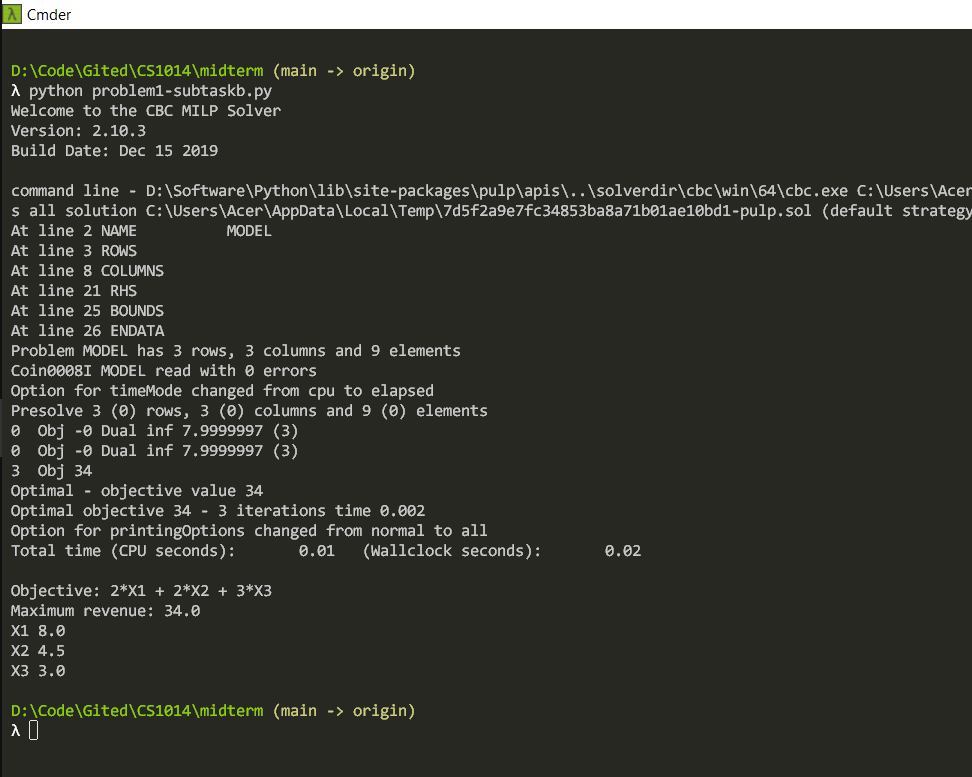
\includegraphics[scale=.65]{img/problem1-console.PNG}
    \caption{Kết quả chạy đoạn chương trình bên trên}
\end{figure}
\noindent Như hình trên, chương trình cho ra kết quả lợi nhuận tối đa $f_{\max} = 34$, đạt được khi $x_1 = 8, x_2 = 4.5, x_3 = 3$, giống với kết quả đã tính ở \ref{problem1-solutiona}.
\\\\
Đến đây ta đã giải xong bài 1.
\pagebreak


\section{Bài 2}
\subsection{Đề bài}
Gọi $a \geq b \geq c \geq d$ là bốn chữ số lớn nhất lấy ra từ mã số sinh viên (MSSV). Xét bài toán quy hoạch tuyến tính sau đây với $x, y \geq 0$ và hàm mục tiêu $f = 29x + 4y \rightarrow \max$:
\begin{equation}
% \label{equation-2}
\left\{ 
\begin{aligned}
ax - dy &\leq 23 \\
cx - by &\geq -22 \\
x + y &\geq 5
\end{aligned}
\right.
\end{equation}
\begin{enumerate}[label=(\alph*)]
\item Hãy giải bài toán quy hoạch tuyến tính trên bằng cách thích hợp.
\item Xác định tất cả các bộ $(a, b, c, d)$ (lấy từ MSSV) có thể có, làm cho bài toán \textbf{vô nghiệm}.
\end{enumerate}
\subsection{Lời giải ý (a)}
Với mã số sinh viên là 19120338, ta có bộ $(a, b, c, d) = (9, 8, 3, 3)$. Khi đó hệ ràng buộc trở thành
\begin{equation}
% \label{equation-2}
\left\{ 
\begin{aligned}
9x - 3y &\leq 23 \\
3x - 8y &\geq -22 \\
x + y &\geq 5
\end{aligned}
\right.
(x, y \geq 0)
\end{equation}
Dễ dàng nhận thấy đây là hệ bất phương trình 2 ẩn và ta có thể dễ dàng giải bằng phương pháp hình học. Miền ràng buộc được biểu diễn như hình sau:
\begin{figure}[H]
    \centering
    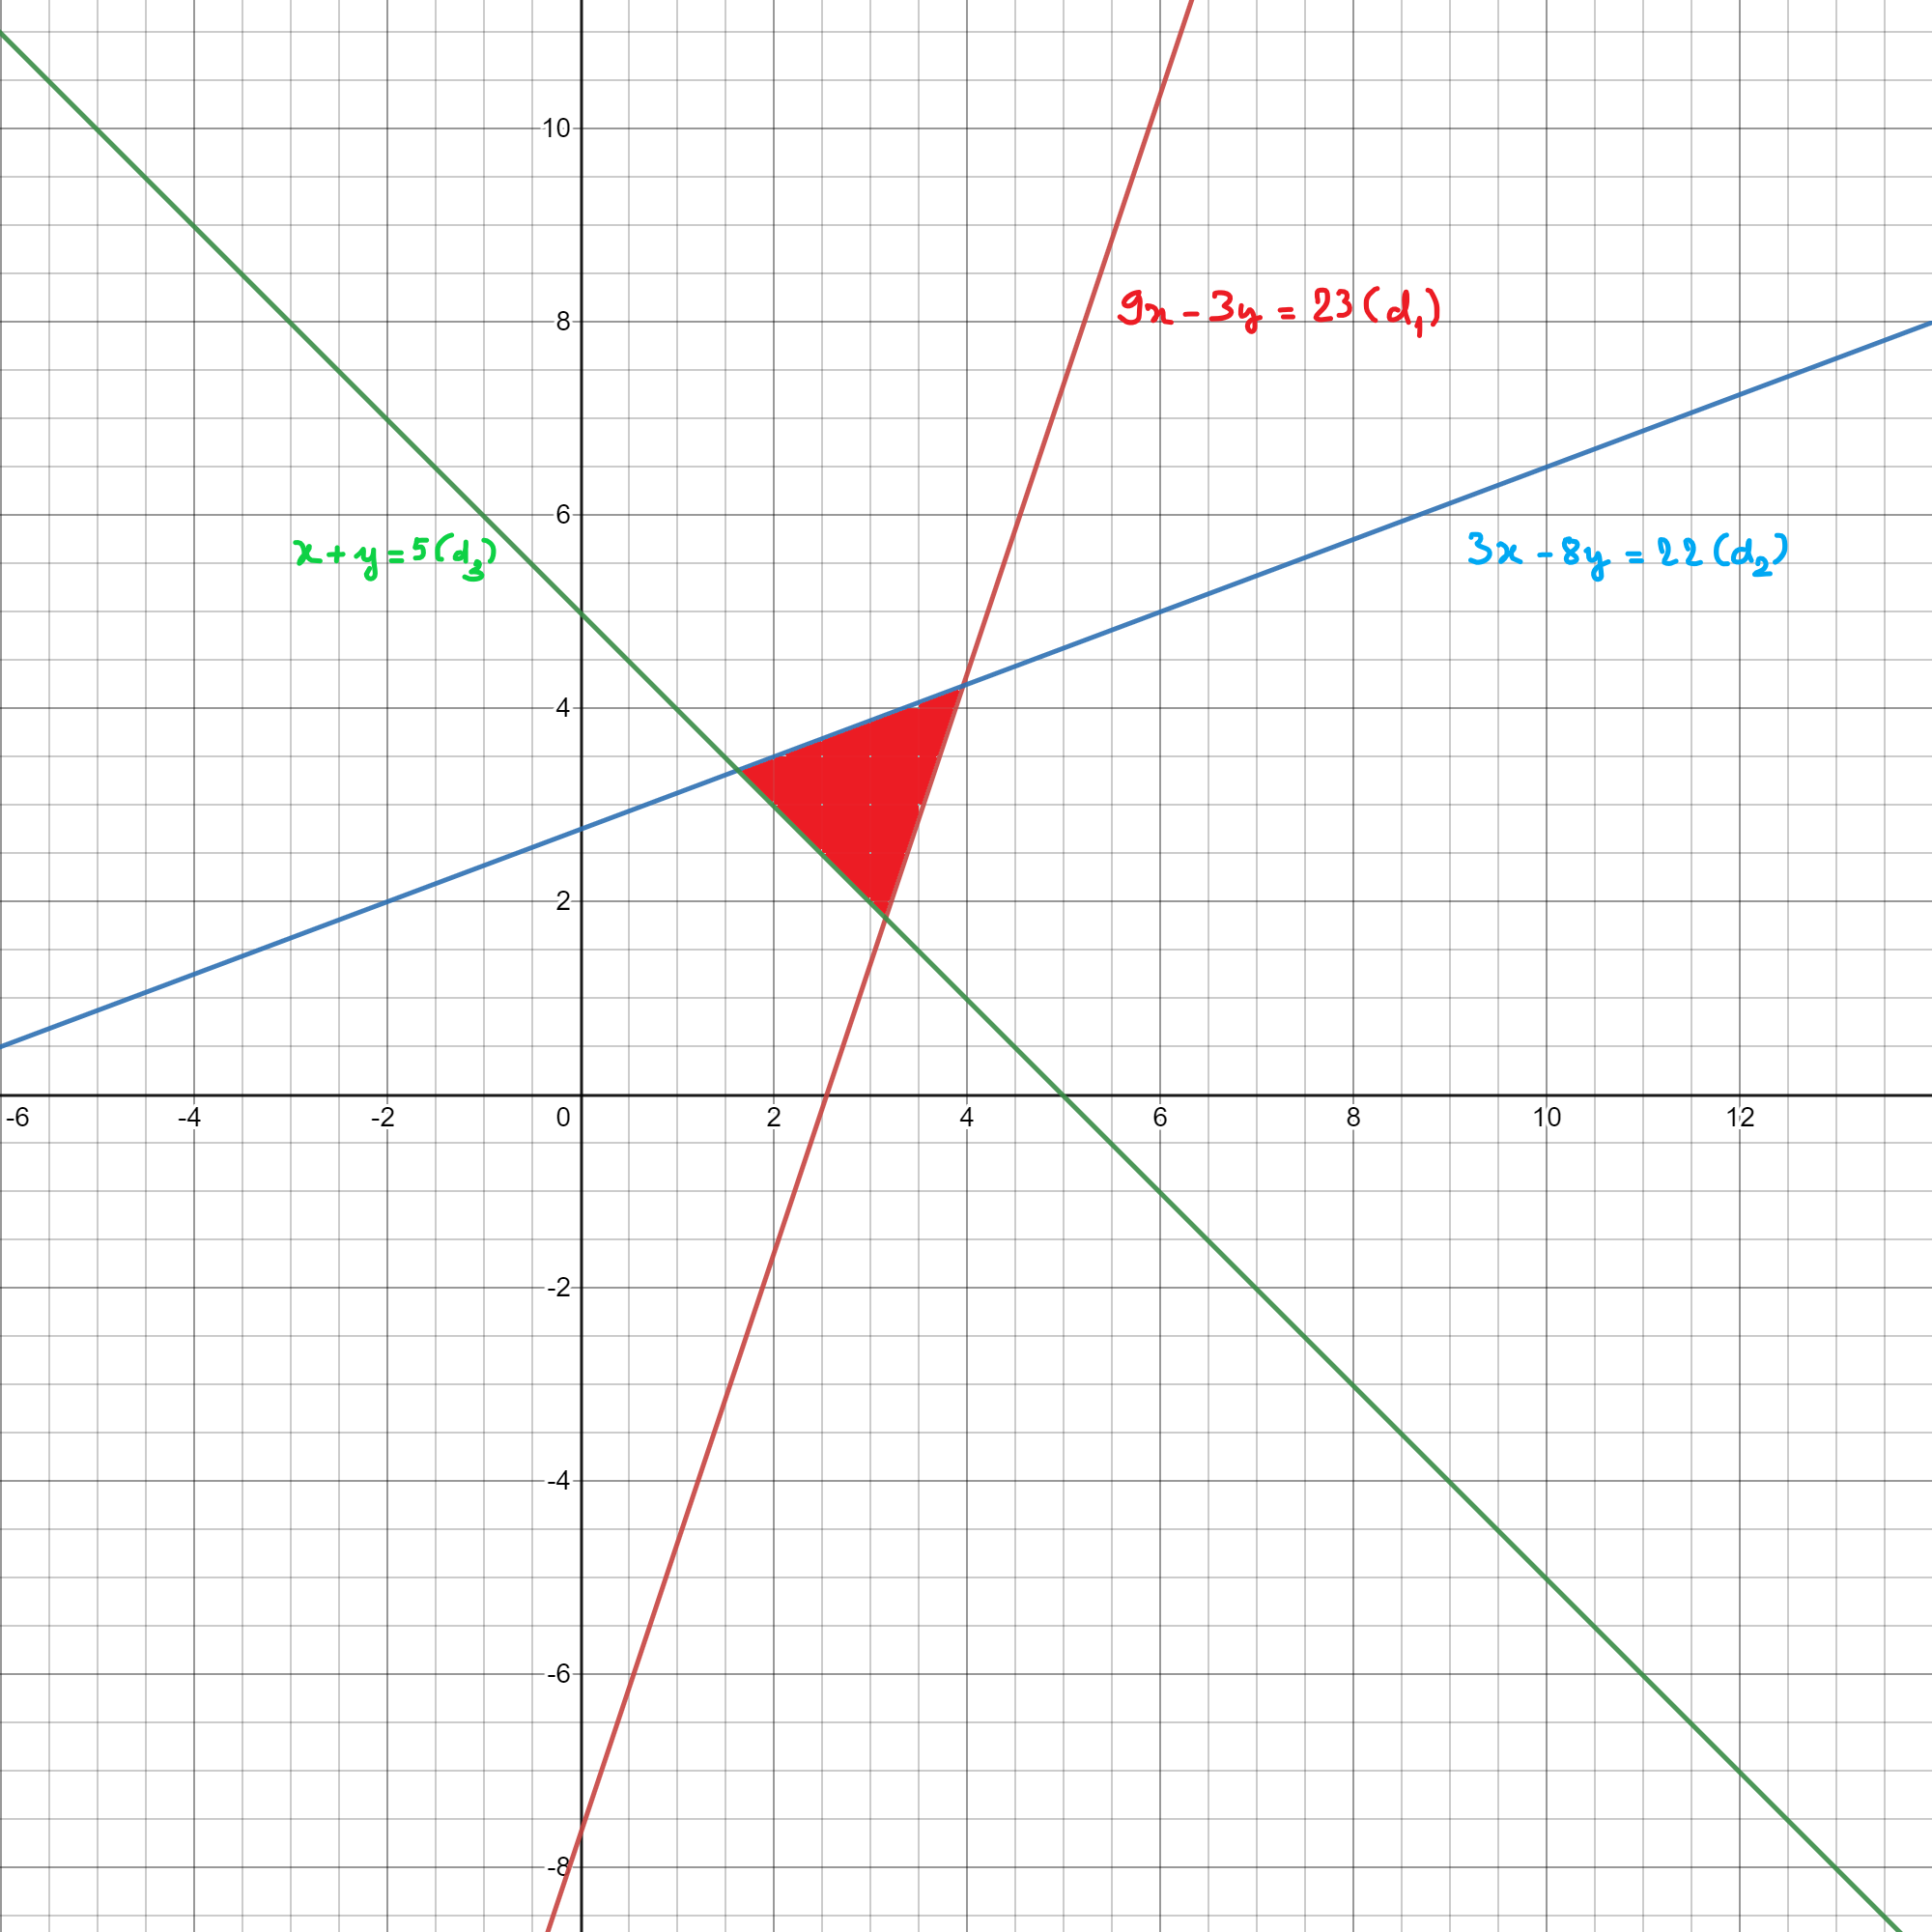
\includegraphics[scale=.2]{img/zone.png}
    \caption{Biểu diễn miền ràng buộc}
\end{figure}
\noindent Dễ dàng nhận thấy miền ràng buộc bị chặn là một tam giác có các đỉnh cực biên:
\begin{itemize}
\item $d_1 \cap d_2$, ta giải hệ
\begin{equation}
% \label{equation-2}
\left\{ 
\begin{aligned}
9x - 3y &= 23 \\
3x - 8y &= -22
\end{aligned}
\right.
\end{equation}
Hệ có 1 nghiệm $\displaystyle \left(\frac{250}{63}, \frac{89}{21}\right)$.
\item $d_1 \cap d_3$, ta giải hệ
\begin{equation}
% \label{equation-2}
\left\{ 
\begin{aligned}
9x - 3y &= 23 \\
x + y &= 5
\end{aligned}
\right.
\end{equation}
Hệ có 1 nghiệm $\displaystyle \left(\frac{19}{6}, \frac{11}{6}\right)$.
\item $d_2 \cap d_3$, ta giải hệ
\begin{equation}
% \label{equation-2}
\left\{ 
\begin{aligned}
3x - 8y &= -22 \\
x + y &= 5
\end{aligned}
\right.
\end{equation}
Hệ có 1 nghiệm $\displaystyle \left(\frac{18}{11}, \frac{37}{11}\right)$.
\end{itemize}
Xét giá trị $f$ tại các đỉnh cực biên, ta có
\begin{itemize}
\item $\displaystyle f\left(\frac{250}{63}, \frac{89}{21}\right) = \frac{8318}{63} \approx 132.03$
\item $\displaystyle f\left(\frac{19}{6}, \frac{11}{6}\right) = \frac{595}{6} \approx 99.16$
\item $\displaystyle f\left(\frac{18}{11}, \frac{37}{11}\right) = \frac{670}{11} \approx 60.9$
\end{itemize}
Vậy phương án tối ưu $\displaystyle f_{\max} = \frac{8318}{63}$, đạt được khi $\displaystyle x = \frac{250}{63}, y = \frac{89}{21}$.
\subsection{Lời giải ý (b)}
Các giá trị $(a, b, c, d)$ lấy từ MSSV theo đề bài $(a \geq b \geq c \geq d)$ sao cho $\displaystyle \frac{a}{c} = \frac{d}{b}$ sẽ làm cho bài toán vô nghiệm.

\begin{proof}
Đặt
$$
\begin{aligned}
&(d_1): ax - dy = 23 \iff y = \frac{a}{d}x - \frac{23}{d} \\
&(d_2): cx - by = -22 \iff y = \frac{c}{b}x + \frac{22}{b} \\
&(d_3): x + y = 5 \iff y = -x + 5
\end{aligned}
$$
Ta nhận xét:
\begin{itemize}
\item $d_3$ có hệ số góc -1 < 0
\item $d_1$ và $d_2$ có hệ số góc $\displaystyle \frac{a}{d}, \frac{c}{b} > 0$ (vì theo dữ kiện đề bài, $a, b, c, d$ lấy từ MSSV nên các giá trị phải là số nguyên nằm trong đoạn $\left[0, 9\right]$; hơn nữa đề bài đã cho điều kiện $a \geq b \geq c \geq d$, nên ta có kết luận trên).
\end{itemize}
Khi đó $d_3$ sẽ luôn cắt $d_1$ và $d_2$ tại 2 giao điểm. Từ đây ta có thể nhận xét, miền ràng buộc $\mathbb{D}$ tạo bởi $d_1, d_2$ và $d_3$ chỉ bị chặn khi $d_1$ cắt $d_2$, hay $\displaystyle \frac{a}{c} \neq \frac{d}{b}$. Vậy, với các giá trị $a, b, c, d \in [0, 9] : a \geq b \geq c \geq d$, bài toán vô nghiệm khi $\displaystyle \frac{a}{c} = \frac{d}{b}$. 
\end{proof}

\noindent Đến đây chúng ta đã giải quyết xong bài 2.
\pagebreak

\section{Bài 3}
\subsection{Đề bài}
Cho $(P)$ là bài toán quy hoạch tuyến tính ba biến $x_1, x_2, x_3$ có hàm mục tiêu là $f(x_1, x_2, x_3) = 2x_1 - x_2 + 4x_3 \rightarrow \min$ với các ràng buộc như sau:
\begin{equation}
\label{equation-4}
\left\{ 
\begin{aligned}
x_1 - x_2 + 2x_3 = 5 \\
2x_1 - x_2 + x_3 \geq 3 
\end{aligned}
\right.
(x_1 \leq 0, x_2 \in \mathbb{R}, x_3 \geq 0)\end{equation}
\begin{enumerate}[label=(\alph*)]
\item Hãy phát biểu bài toán đối ngẫu $(D)$ của bài toán $(P)$. So sánh tính khả thi của việc áp dụng phương pháp hình học vào giải $(P)$ và giải $(D)$.
\item Người ta đã tính được phương án tối ưu của $(D)$ ứng với hai số 0 và 1 nhưng chưa rõ giá trị nào ứng với biến nào. \textbf{Không giải trực tiếp bài toán $(P)$}, mô tả rõ các bước xác định phương án tối ưu cho bài toán $(P)$ từ $(D)$.
\end{enumerate}
\subsection{Lời giải ý (a)}
Qua quan sát:
\begin{itemize}
    \item Bài toán ban đầu có 2 ràng buộc và 3 biến, vậy bài toán đối ngẫu phải có 3 ràng buộc và 2 biến.
    \item Hàm mục tiêu ban đầu là tìm min, vậy hàm mục tiêu đối ngẫu phải tìm max.
\end{itemize}
Khi đó ta có thể tìm ra bài toán đối ngẫu $(D)$:
\begin{equation}
\label{equation-5}
\left\{ 
\begin{aligned}
y_1 + 2y_2 &\geq 2 \\
-y_1 - y_2 &= -1 \\
2y_1 + y_2 &\leq 4
\end{aligned}
\right.
(y_1 \in \mathbb{R}, y_2 \geq 0)
\end{equation}
với hàm mục tiêu $g = 5y_1 + 3y_2 \rightarrow \max$.
\\\\
Dễ dàng nhận thấy đây là hệ bất phương trình bậc 1, mỗi ràng buộc chỉ có tối đa 2 ẩn nên ta có thể dễ dàng giải bằng phương pháp hình học. Ngược lại, với bài toán ban đầu ta khó có thể giải bằng phương pháp hình học, vì để giải ta cần không gian 3 chiều để biểu diễn 3 biến trong mỗi ràng buộc.
\subsection{Lời giải ý (b)}
\begin{theorem}\label{strong-theorem}
Nếu tồn tại hai phương án chấp nhận được $x^*, y^*$ của bài toán gốc và bài toán đối ngẫu mà $(x^*)^{\intercal}c = (y^*)^{\intercal}b$ thì ta có thể hiểu đẳng thức xảy ra và đó cũng là phương án tối ưu cho cả hai bài toán.\cite{lplu-2021}
\end{theorem}
\noindent Vì yêu cầu của đề bài là xác định phương án tối ưu của $(P)$ từ $(D)$ mà không qua tính toán $(P)$; mặt khác ta đã biết được bài toán $(D)$ có phương án tối ưu $g_{\max}$ đạt được với $(y_1, y_2) = (0, 1)$ hoặc $(1, 0)$. Vậy ta tiến hành xét các phương  án có thể có:
\begin{itemize}
\item Xét phương án $(1, 0)$, khi đó $y_1 = 1, y_2 = 0$. Điều này mâu thuẫn với ràng buộc thứ 1 trong \ref{equation-5}: $y_1 + 2y_2 = 1 + 2\times 0 = 1 \ngeq 2$.
\item Xét phương án $(0, 1)$, khi đó $y_1 = 0, y_2 = 1$. Phương án này thỏa các ràng buộc.
\end{itemize}
Khi đó: $g_{\max} = 5y_1 + 3y_2 = 5 \times 0 + 3 \times 1 = 3$. Vậy bài toán đối ngẫu có $g_{\max} = 3$ khi $y_1 = 0, y_2 = 1$. Từ định lý \ref{strong-theorem}, điều này cũng có nghĩa là $g_{\max} = f_{\min} = 3$. Dùng định lý độ lệch bù:
\begin{itemize}
\item Do $y_2 = 1$ khác 0 nên dấu bằng trong ràng buộc 2 (trong hệ ràng buộc \ref{equation-4}) phải xảy ra, nghĩa là $2x_1 - x_2 + x_3 = 3$.
\item Thay bộ $(0, 1)$ vào ràng buộc 3 (trong hệ ràng buộc \ref{equation-5}) thì dấu bằng không xảy ra. Vì vậy bắt buộc $x_3 = 0$.

\end{itemize}
Đến đây ta có hệ 3 phương trình 3 ẩn:
\begin{equation}
\left\{ 
\begin{aligned}
x_3 = 0 \\
2x_1 - x_2 + x_3 = 3 \\
x_1 - x_2 + 2x_3 = 5
\end{aligned}
\right.
\iff 
\left\{ 
\begin{aligned}
x_1 - x_2 &= 5 \\
2x_1 - x_2 &= 3 \\
x_3 &= 0
\end{aligned}
\right.
\iff
\left\{ 
\begin{aligned}
x_1 &= -2 \\
x_2 &= -7 \\
x_3 &= 0
\end{aligned}
\right.
\end{equation}
Kiểm tra lại với hàm mục tiêu: $f(x_1, x_2, x_3) = f(-2, -7, 0) = 3$, đây cũng là $f_{\min}$ như đã nêu bên trên. Dù ta không tính toán $(P)$, nhưng thông qua bài toán đối ngẫu $(D)$ ta đã tính toán được phương án tối ưu $f_{\min} = 3$ xảy ra khi $x_1 = -2, x_2 = -7, x_3 = 0$.
\\\\
Đến đây chúng ta đã giải xong bài 3.
\cleardoublepage
\phantomsection
\addcontentsline{toc}{section}{Tài liệu}
\bibliographystyle{plain}
\bibliography{sample}

\end{document}